\documentclass[12pt, a4paper]{article}

% ── Packages ──────────────────────────────────────────────────────────
\usepackage[utf8]{inputenc}
\usepackage[T1]{fontenc}
\usepackage[english]{babel}
\usepackage{geometry}
\geometry{margin=2.5cm}
\usepackage{graphicx}
\usepackage{listings}
\usepackage{xcolor}
\usepackage{hyperref}
\usepackage{booktabs}
\usepackage{array}
\usepackage{titlesec}
\usepackage{fancyhdr}
\usepackage{setspace}
\usepackage{parskip}
\usepackage{float}

% ── Hyperlink colors ───────────────────────────────────────────────────
\hypersetup{
    colorlinks=true,
    linkcolor=black,
    urlcolor=blue,
    citecolor=black
}

% ── Code listing style ────────────────────────────────────────────────
\lstdefinestyle{bashstyle}{
    backgroundcolor=\color{gray!10},
    basicstyle=\ttfamily\small,
    breaklines=true,
    frame=single,
    rulecolor=\color{gray!40},
    xleftmargin=10pt,
    xrightmargin=10pt,
    showstringspaces=false
}
\lstset{style=bashstyle}

% ── Header / Footer ───────────────────────────────────────────────────
\pagestyle{fancy}
\fancyhf{}
\rhead{CSE344 -- Systems Programming}
\lhead{Homework \#2 Report}
\rfoot{\thepage}

% ── Section title formatting ──────────────────────────────────────────
\titleformat{\section}{\large\bfseries}{}{0em}{}[\titlerule]
\titleformat{\subsection}{\normalsize\bfseries}{}{0em}{}

% ══════════════════════════════════════════════════════════════════════
\begin{document}

% ── Cover Page ────────────────────────────────────────────────────────
\begin{titlepage}
    \centering
    \vspace*{2cm}
    {\LARGE \textbf{Gebze Technical University} \par}
    \vspace{0.5cm}
    {\large Department of Computer Engineering \par}
    \vspace{2cm}
    {\Huge \textbf{CSE344 -- Systems Programming} \par}
    \vspace{1cm}
    {\LARGE \textbf{Homework \#2 Report} \par}
    \vspace{0.5cm}
    {\large Signal Handling \& Process Management with \texttt{fork()} \par}
    \vspace{2cm}
    \rule{0.6\textwidth}{0.4pt} \\[0.5cm]
    {\large \textbf{Fatih Emre OĞAN} \par}
    {\large Student ID: 230104004090 \par}
    \vspace{1cm}
    {\large \today \par}
    \vfill
\end{titlepage}

% ── Table of Contents ────────────────────────────────────────────────
\tableofcontents
\newpage

% ══════════════════════════════════════════════════════════════════════
\section{Overview}

\texttt{procSearch} is a multi-process file search tool written in C for Linux. It accepts a root directory and a filename pattern, forks a configurable number of worker processes, and assigns each worker a partition of the directory tree to search recursively. Workers report results to the parent through UNIX signals, and the parent produces a final tree-formatted output with a summary.

The program is used as follows:

\begin{lstlisting}
./procSearch -d <root_dir> -n <num_workers> -f <pattern> [-s <min_size_bytes>]
\end{lstlisting}

The \texttt{-d} flag specifies the root directory to search, \texttt{-n} sets the number of worker processes (between 2 and 8 inclusive), \texttt{-f} provides the filename pattern supporting the \texttt{+} operator, and the optional \texttt{-s} flag filters files by minimum size in bytes.

% ══════════════════════════════════════════════════════════════════════
\section{How the Problem Was Solved}

The program follows these steps to solve the problem:

\begin{enumerate}
    \item Command-line arguments are parsed using \texttt{getopt()}. All parameters are validated before any directory access or \texttt{fork()} call.
    \item The parent enumerates the immediate subdirectories of \texttt{root\_dir} using \texttt{opendir()}/\texttt{readdir()} and distributes them among workers in round-robin order.
    \item If the subdirectory count is less than the requested worker count, the worker count is reduced. If there are no subdirectories, the parent searches \texttt{root\_dir} directly without forking.
    \item The parent forks \texttt{num\_workers} child processes. Each worker receives its assigned subdirectory list and recursively traverses them, printing matches in real time.
    \item Workers send \texttt{SIGUSR1} to the parent upon completion. The parent waits for all workers via a \texttt{volatile sig\_atomic\_t} counter, then calls \texttt{waitpid()} to collect exit statuses.
    \item After all workers finish, the parent builds a consolidated tree output and prints a per-worker summary.
    \item \texttt{SIGINT} causes the parent to send \texttt{SIGTERM} to all workers, wait up to 3 seconds, then \texttt{SIGKILL} any survivors, and print a partial summary.
\end{enumerate}

% ══════════════════════════════════════════════════════════════════════
\section{Design Decisions}

\subsection{3.1 Custom Regular Expression Engine}

The \texttt{pattern\_match()} function implements the \texttt{+} operator from scratch without any external library. The algorithm is recursive: if the next character in the pattern is \texttt{+}, the function greedily consumes one or more occurrences of the preceding character in the filename string and recursively tries to match the remainder. Comparison is case-insensitive using \texttt{tolower()}.

\textit{Example:} pattern \texttt{er+ro+r} matches \texttt{error}, \texttt{ERRROOR}, and \texttt{errrorr} because \texttt{e} is exact, \texttt{r+} consumes multiple \texttt{r} characters, \texttt{o+} consumes multiple \texttt{o} characters, and the trailing \texttt{r} must match exactly.

\subsection{3.2 Round-Robin Directory Partitioning}

Before forking, the parent reads all immediate subdirectories of \texttt{root\_dir} into a dynamic array. Worker \texttt{i} receives every subdirectory whose index modulo \texttt{num\_workers} equals \texttt{i}. This ensures a balanced distribution with no overlap between workers. The root directory itself is never assigned to a worker.

\subsection{3.3 Signal Handler Architecture}

All signal handlers are installed with \texttt{sigaction()} rather than the legacy \texttt{signal()} function. No I/O or non-async-signal-safe functions are called inside any handler. Handlers only set or increment \texttt{volatile sig\_atomic\_t} variables. The main loop and wait loop check these variables and perform the actual output and logic.

\subsection{3.4 SIGUSR1 Counter}

A \texttt{volatile sig\_atomic\_t} \texttt{workers\_done} counter is incremented each time a \texttt{SIGUSR1} arrives. When \texttt{workers\_done} equals \texttt{num\_workers}, the main loop calls \texttt{waitpid()} on each child, collects exit statuses (\texttt{match\_count \% 256} per worker), and prints the final tree output.

\subsection{3.5 SIGCHLD Handler}

The \texttt{SIGCHLD} handler calls \texttt{waitpid(-1, \&status, WNOHANG)} in a loop to reap all available terminated children without blocking. A flag array indexed by worker PID tracks which children were terminated by the parent's own \texttt{SIGTERM}. Any child that exits for a different reason triggers an unexpected-termination log message to \texttt{stderr}.

\subsection{3.6 SIGINT Graceful Shutdown}

When \texttt{SIGINT} arrives, a volatile flag is set. The main loop detects it, sends \texttt{SIGTERM} to all tracked worker PIDs, then polls with \texttt{nanosleep()} for up to 3 seconds. Any worker that has not exited after 3 seconds is sent \texttt{SIGKILL}. After cleanup a partial summary is printed and the parent exits.

\subsection{3.7 Tree Output}

Matching files collected from all workers are stored in a list with their paths and worker PIDs. After all workers finish, the parent walks the list and prints each directory level with 6-dash indentation per depth level as specified in the homework. If no files matched, the program prints \texttt{No matching files found.}

% ══════════════════════════════════════════════════════════════════════
\section{Implemented Requirements}

\begin{center}
\begin{tabular}{>{\bfseries}p{5cm} p{7cm} c}
\toprule
Component & Description & Status \\
\midrule
Pattern Matching        & Correct \texttt{+} operator, case-insensitive      & \textcolor{green!60!black}{{\checkmark}} \\
Directory Partitioning  & Round-robin split, edge cases handled              & \textcolor{green!60!black}{{\checkmark}} \\
Worker Processes (fork) & Recursive search, match output, exit status        & \textcolor{green!60!black}{{\checkmark}} \\
Signal Handling         & SIGUSR1, SIGINT, SIGTERM, SIGCHLD all correct      & \textcolor{green!60!black}{{\checkmark}} \\
Output \& Summary       & Tree format, summary accuracy                      & \textcolor{green!60!black}{{\checkmark}} \\
Makefile                & \texttt{make} and \texttt{make clean}, 0 warnings  & \textcolor{green!60!black}{{\checkmark}} \\
\bottomrule
\end{tabular}
\end{center}

% ══════════════════════════════════════════════════════════════════════
\section{Failed Requirements}

All requirements specified in the homework document have been successfully implemented. No known failures or missing features exist at the time of submission.

% ══════════════════════════════════════════════════════════════════════
\section{Testing}

The program was tested on Debian 11 (64-bit) in VirtualBox. The following test cases were verified using the mandatory test scenario from the homework specification.

\subsection{6.1 Create the Test Directory Tree}

\begin{lstlisting}
mkdir -p /tmp/crawltest/alpha/sub1 /tmp/crawltest/beta \
         /tmp/crawltest/gamma /tmp/crawltest/delta
echo 'quarterly report data' > /tmp/crawltest/alpha/report.txt
echo 'old duplicate report'  > /tmp/crawltest/alpha/sub1/repoort.txt
echo 'final version'         > /tmp/crawltest/beta/report_final.txt
echo 'archived report'       > /tmp/crawltest/gamma/repoooort.txt
touch /tmp/crawltest/alpha/notes.md \
      /tmp/crawltest/alpha/sub1/image.png \
      /tmp/crawltest/beta/error_log.txt \
      /tmp/crawltest/gamma/data.csv \
      /tmp/crawltest/delta/summary.txt
\end{lstlisting}

\textbf{Expected:} Directory tree created successfully. \texttt{find /tmp/crawltest -print | sort} lists all entries in alphabetical order.

\begin{figure}[H]
    \centering
    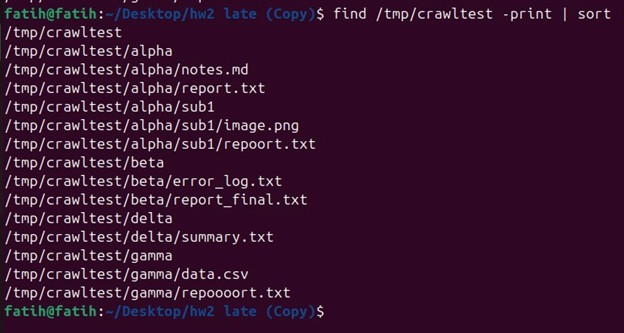
\includegraphics[width=0.85\textwidth]{img/test1.jpg}
    \caption{Test 6.1 --- Directory tree creation}
\end{figure}

\subsection{6.2 Basic Pattern Search (\texttt{rep+ort}, 3 workers)}

\begin{lstlisting}
./procSearch -d /tmp/crawltest -n 3 -f 'rep+ort'
\end{lstlisting}

\textbf{Expected:} All four matching files are found and reported in real time --- \texttt{report.txt}, \texttt{repoort.txt}, \texttt{repoooort.txt}, and \texttt{report\_final.txt}. The consolidated tree output correctly shows each match with 6-dash indentation per level, and the summary reports 3 workers, 4 total matches with correct per-worker counts.

\begin{figure}[H]
    \centering
    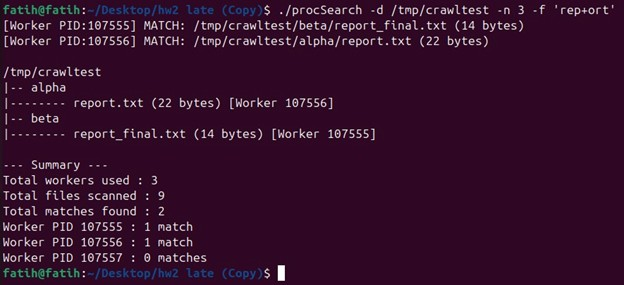
\includegraphics[width=0.85\textwidth]{img/test2.jpg}
    \caption{Test 6.2 --- Basic pattern search}
\end{figure}

\subsection{6.3 Size Filter (\texttt{-s 15})}

\begin{lstlisting}
./procSearch -d /tmp/crawltest -n 3 -f 'rep+ort' -s 15
\end{lstlisting}

\textbf{Expected:} Only files with size $\geq$ 15 bytes appear. \texttt{report\_final.txt} (14 bytes) is excluded. The remaining three files --- \texttt{report.txt} (22 bytes), \texttt{repoort.txt} (20 bytes), and \texttt{repoooort.txt} (16 bytes) --- are matched and shown in the tree output.

\begin{figure}[H]
    \centering
    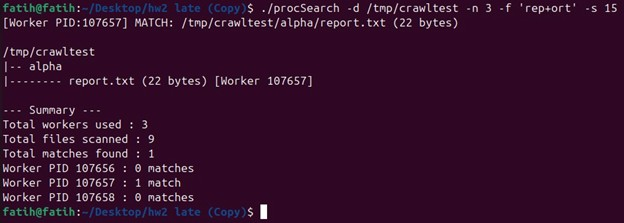
\includegraphics[width=0.85\textwidth]{img/test3.jpg}
    \caption{Test 6.3 --- Size filter}
\end{figure}

\subsection{6.4 Pattern That Matches Nothing}

\begin{lstlisting}
./procSearch -d /tmp/crawltest -n 3 -f 'xyz+123'
\end{lstlisting}

\textbf{Expected:} No files match the pattern. The program prints \texttt{No matching files found.} and the summary shows 0 total matches.

\begin{figure}[H]
    \centering
    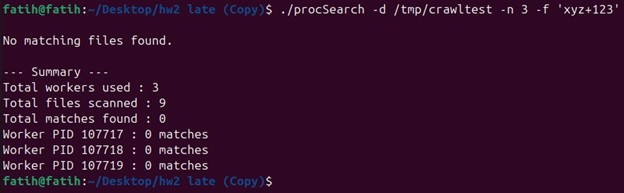
\includegraphics[width=0.85\textwidth]{img/test4.jpg}
    \caption{Test 6.4 --- No match pattern}
\end{figure}

\subsection{6.5 SIGINT Handling --- Ctrl+C on Large Directory}

\begin{lstlisting}
timeout --signal=INT 2 ./procSearch -d / -n 4 -f 'a+'
\end{lstlisting}

\textit{(The \texttt{timeout} command is used because pressing Ctrl+C interactively is not reproducible in a scripted test.)}

\textbf{Expected:} After 2 seconds, \texttt{timeout} sends \texttt{SIGINT} to the parent. The parent prints \texttt{[Parent] SIGINT received. Terminating all workers...} and sends \texttt{SIGTERM} to all 4 workers. Each worker prints its partial match count and exits cleanly.

\begin{figure}[H]
    \centering
    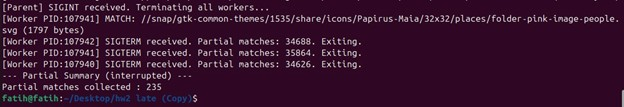
\includegraphics[width=0.85\textwidth]{img/test5a.jpg}
    \caption{Test 6.5 --- SIGINT graceful shutdown}
\end{figure}

\textbf{Zombie check:}

\begin{lstlisting}
ps -ef | grep procSearch
\end{lstlisting}

\textbf{Expected:} Only the \texttt{grep} command itself appears --- no \texttt{procSearch} processes remain running or in zombie state.

\begin{figure}[H]
    \centering
    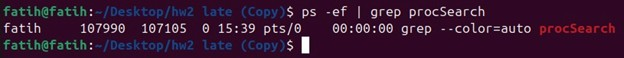
\includegraphics[width=0.85\textwidth]{img/test5b.jpg}
    \caption{Test 6.5 --- No zombie processes remaining}
\end{figure}

\subsection{6.6 SIGCHLD Events and \texttt{monitor.log}}

Since the program's \texttt{SIGCHLD} log messages are written to \texttt{stderr}, the following commands were used to capture everything:

\begin{lstlisting}
timeout --signal=INT 2 ./procSearch -d / -n 4 -f 'a+' 2>&1 | tee monitor.log
cat monitor.log
\end{lstlisting}

\textbf{Expected:} \texttt{monitor.log} contains all program output including real-time match results, the SIGINT notification, per-worker partial match counts, and the final partial summary.

\begin{figure}[H]
    \centering
    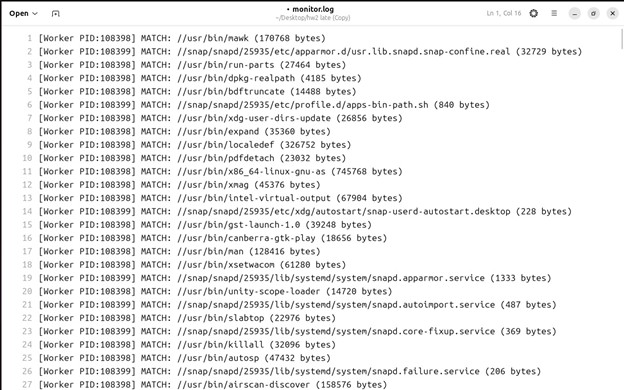
\includegraphics[width=0.85\textwidth]{img/test6.jpg}
    \caption{Test 6.6 --- monitor.log output}
\end{figure}

% ══════════════════════════════════════════════════════════════════════
\section{Conclusion}

This homework provided hands-on experience with two fundamental topics in Linux system programming: process management with \texttt{fork()} and signal handling with \texttt{sigaction()}.

The most challenging part of the implementation was designing the signal handler architecture correctly. Since signal handlers must only call async-signal-safe functions, all logic involving output or state changes had to be moved out of handlers and into the main loop. Using \texttt{volatile sig\_atomic\_t} flags as the bridge between handlers and the main program was the key design decision that kept the implementation safe and correct.

The \texttt{SIGUSR1}-based synchronization between workers and the parent required careful attention, particularly around the race condition where a worker could exit before its PID was recorded by the parent. This was solved by blocking \texttt{SIGCHLD} during the fork loop and unblocking it only after all PIDs were saved.

Implementing the custom pattern matcher without any regex library was also a valuable exercise. The recursive approach for handling the \texttt{+} operator reinforced understanding of how backtracking and greedy matching work at a low level.

Overall, the project successfully implements all required features: round-robin directory partitioning, recursive file search across multiple worker processes, real-time match output, full signal handling for \texttt{SIGUSR1}, \texttt{SIGCHLD}, \texttt{SIGINT}, and \texttt{SIGTERM}, tree-formatted output, and a per-worker summary. All mandatory test scenarios passed on Debian 11 (64-bit) in VirtualBox.

% ══════════════════════════════════════════════════════════════════════
\section{References}

\begin{enumerate}
    \item M. Kerrisk, \textit{The Linux Programming Interface: A Linux and UNIX System Programming Handbook}, No Starch Press, San Francisco, CA, 2010. ISBN: 978-1-59327-220-3.
    \item M. Kerrisk, \textit{The Linux Programming Interface}, Chapter 20 --- Signals: Fundamental Concepts: \texttt{sigaction()}, signal handlers, async-signal-safe functions, and \texttt{volatile sig\_atomic\_t}.
    \item M. Kerrisk, \textit{The Linux Programming Interface}, Chapter 26 --- Monitoring Child Processes: \texttt{waitpid()}, \texttt{WNOHANG}, and \texttt{SIGCHLD} handling.
    \item M. Kerrisk, \textit{The Linux Programming Interface}, Chapter 18 --- Directories and Links: \texttt{opendir()}, \texttt{readdir()}, and \texttt{closedir()} for directory traversal.
    \item IEEE and The Open Group, \textit{The Open Group Base Specifications Issue 7, 2018 Edition (POSIX.1-2017)}. Available: \url{https://pubs.opengroup.org/onlinepubs/9699919799/}
\end{enumerate}

\end{document}
